% EvidenceGuard-SOC figure snippets — paste into the matching sections.
% Figures are generated by evidenceguard/generate_figures.py (PDF preferred for print).

% --- Chapter 4, Section 4.2 (PCEM), after SHA-256 paragraph ---
\begin{figure}[htbp]
  \centering
  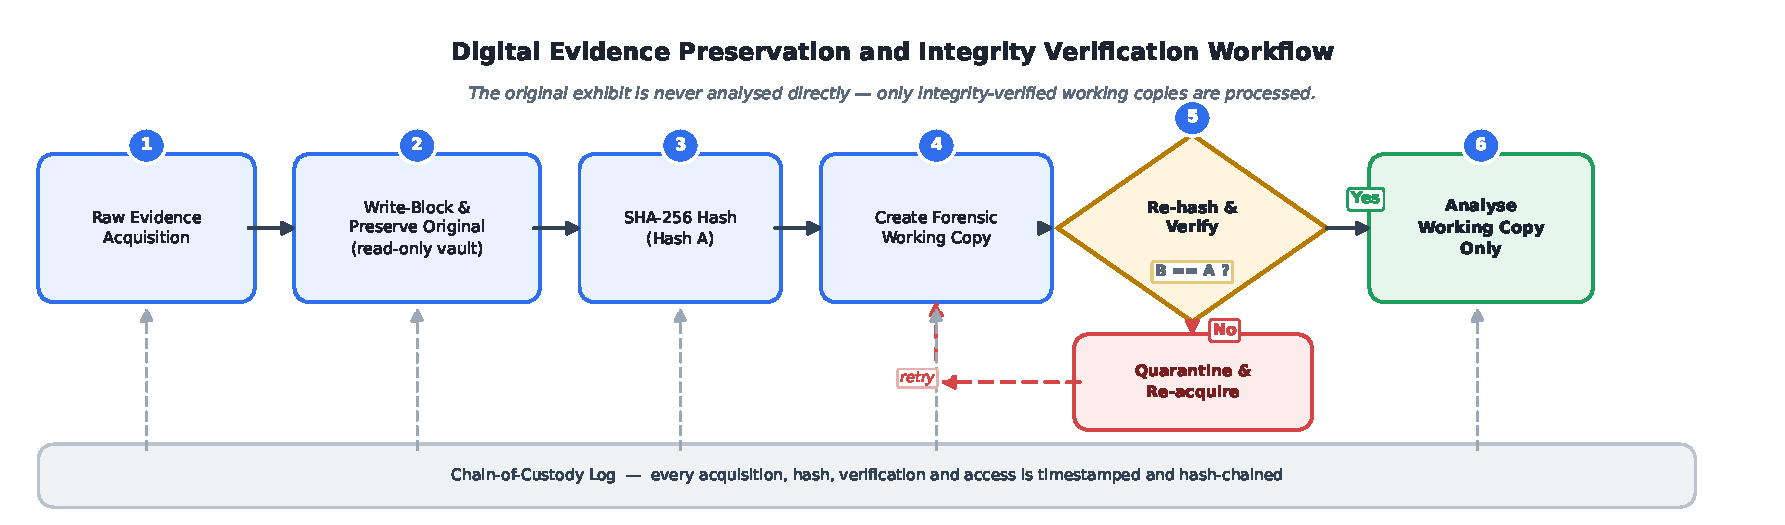
\includegraphics[width=\textwidth]{figures/fig4_2_digital_evidence_preservation_workflow.pdf}
  \caption{Digital Evidence Preservation and Integrity Verification Workflow.}
  \label{fig:evidence-preservation-workflow}
\end{figure}

% --- Chapter 4, Section 4.4 (CCVA), after calibration/ECE explanation ---
\begin{figure}[htbp]
  \centering
  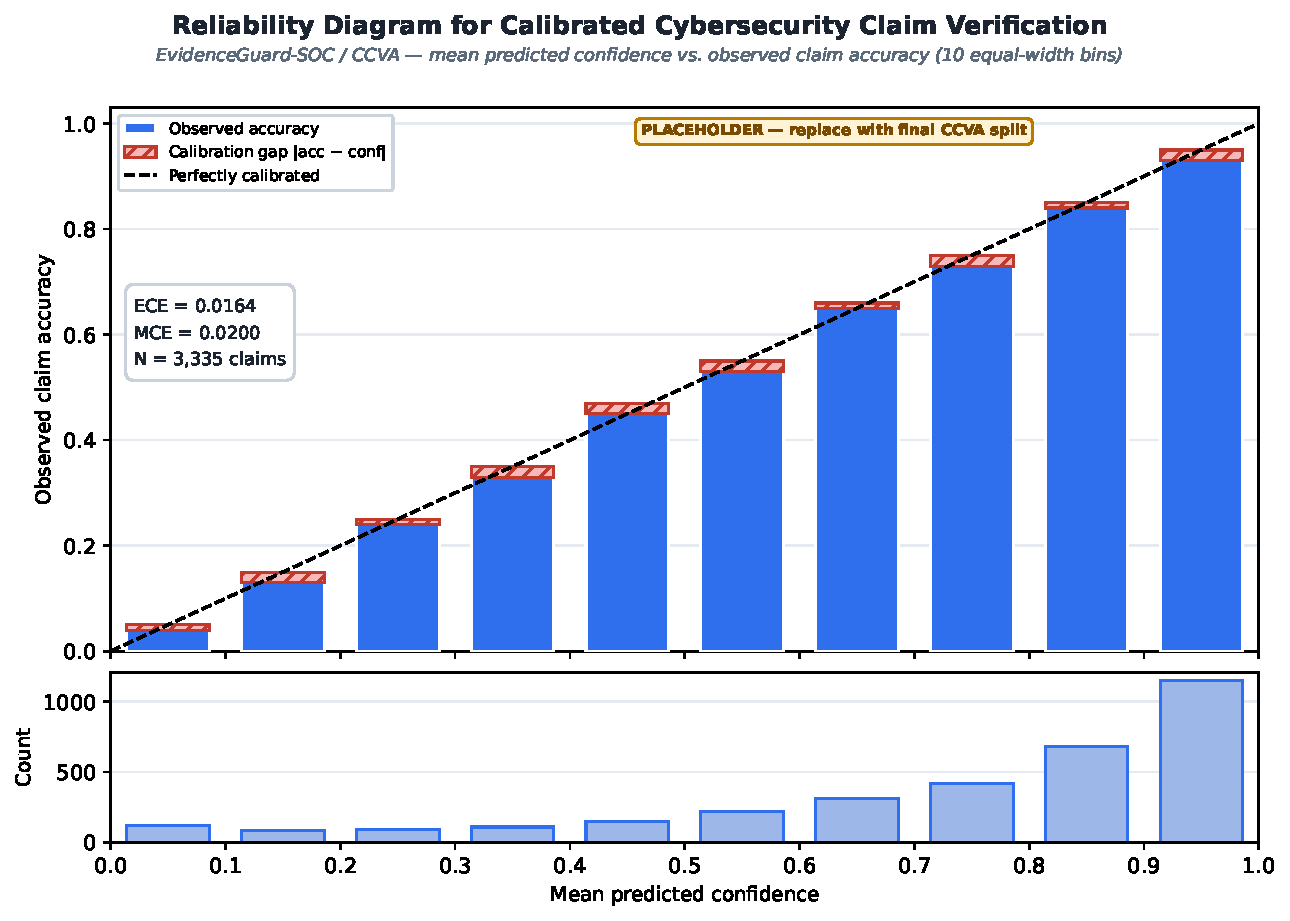
\includegraphics[width=0.92\textwidth]{figures/fig4_4_reliability_diagram_ccva.pdf}
  \caption{Reliability Diagram for Calibrated Cybersecurity Claim Verification.}
  \label{fig:ccva-reliability-diagram}
\end{figure}

% --- Chapter 4, Section 4.5 (RCRA), after the policy-outcome table ---
\begin{figure}[htbp]
  \centering
  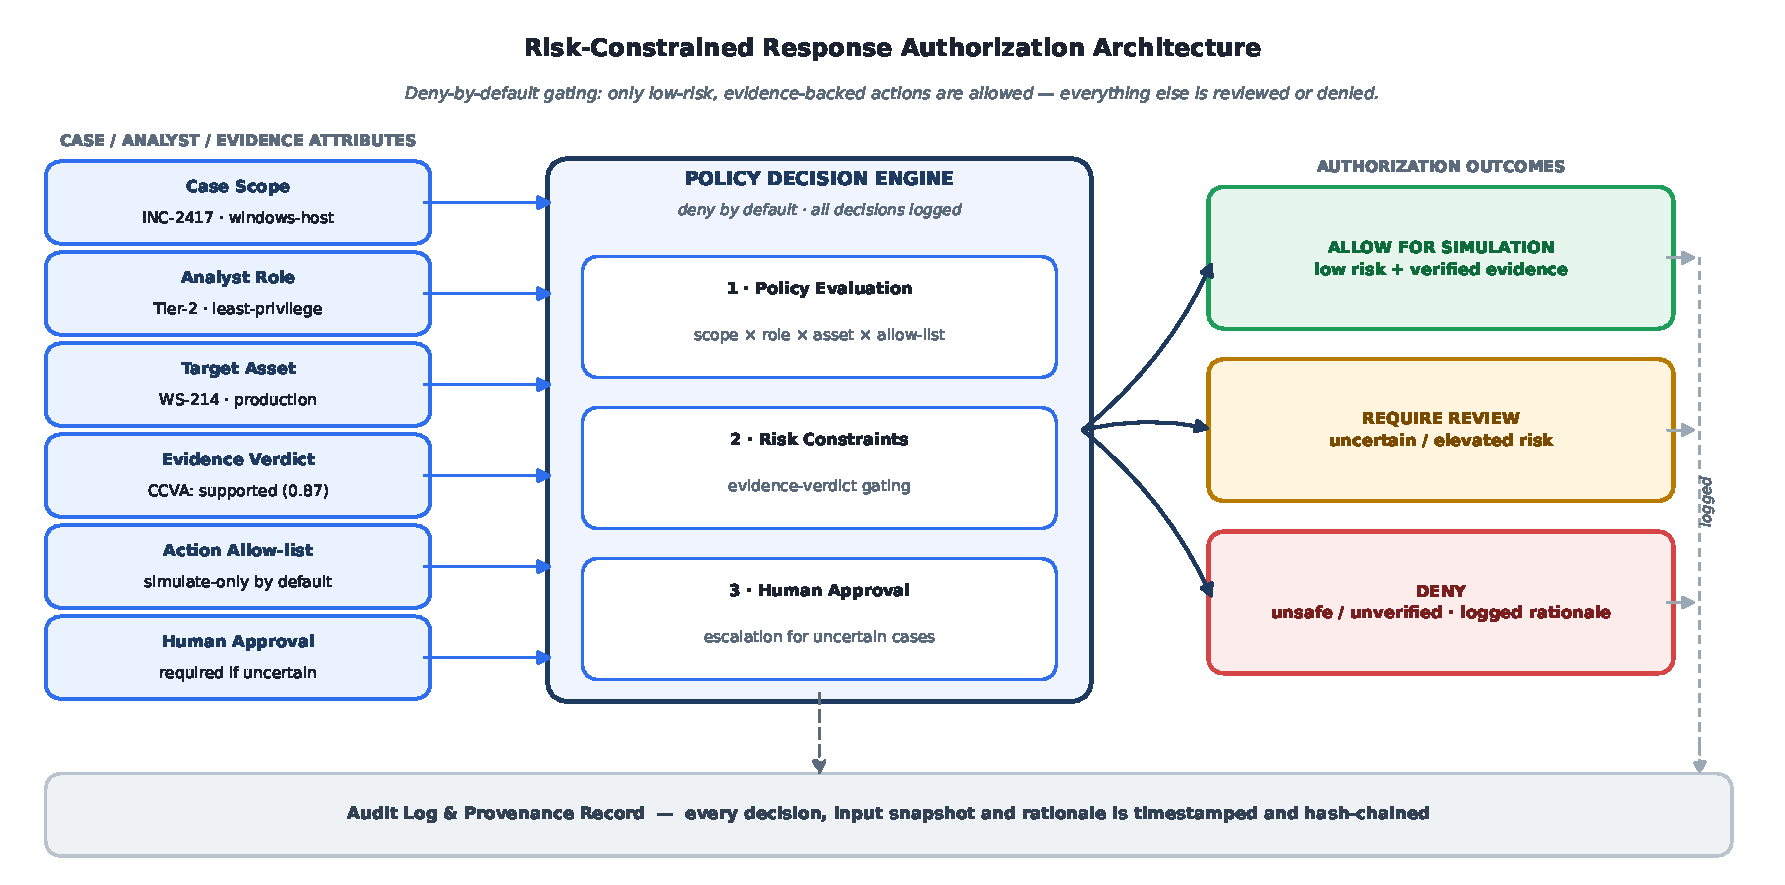
\includegraphics[width=\textwidth]{figures/fig4_5_response_authorization_rcra.pdf}
  \caption{Risk-Constrained Response Authorization Architecture.}
  \label{fig:response-authorization-architecture}
\end{figure}

% --- Chapter 5, Section 5.2 (Temporal Evidence Graph), after nodes/edges explanation ---
\begin{figure}[htbp]
  \centering
  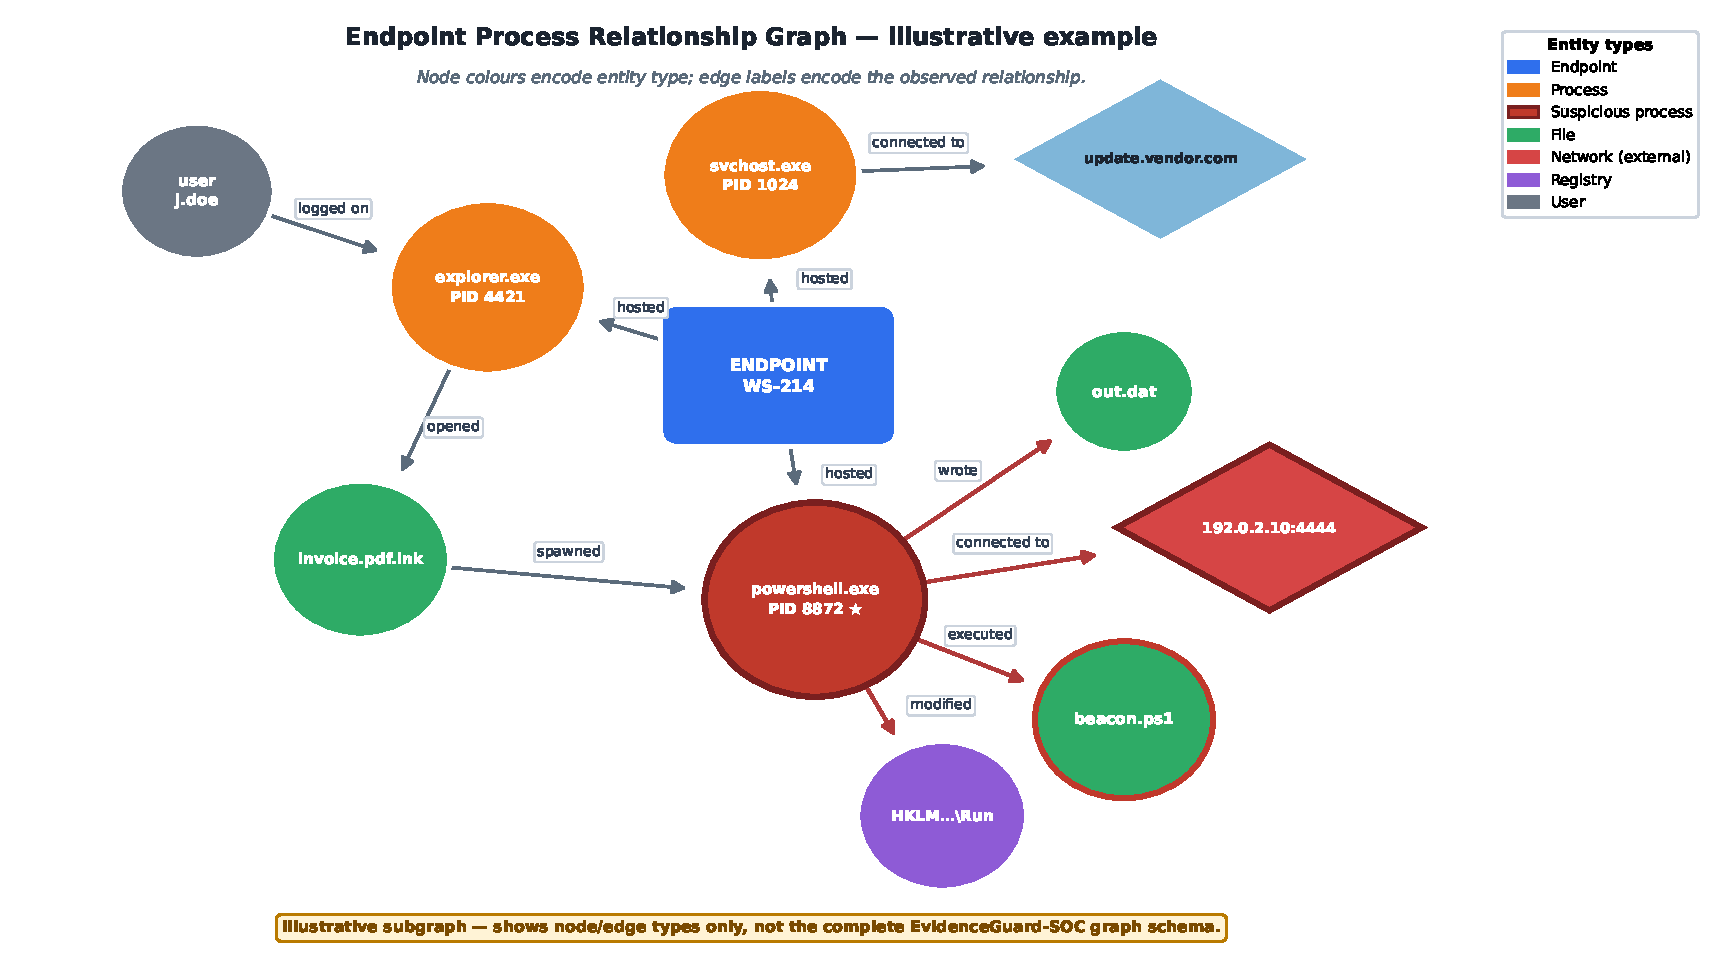
\includegraphics[width=\textwidth]{figures/fig5_2_endpoint_process_graph.pdf}
  \caption{Example of an Endpoint Process Relationship Graph.
  Illustrative subgraph showing node and edge types; not the complete
  EvidenceGuard-SOC graph schema.}
  \label{fig:endpoint-process-graph}
\end{figure}
